%==============================================================================
% Sjabloon poster bachproef
%==============================================================================
% Gebaseerd op document class `a0poster' door Gerlinde Kettl en Matthias Weiser
% Aangepast voor gebruik aan HOGENT door Jens Buysse en Bert Van Vreckem

\documentclass[a0,portrait]{hogent-poster}

% Info over de opleiding
\course{Bachelorproef}
\studyprogramme{toegepaste informatica}
\academicyear{2022-2023}
\institution{Hogeschool Gent, Valentin Vaerwyckweg 1, 9000 Gent}

% Info over de bachelorproef
\title{Automatische productherkenning in \\ Vlaamse supermarkten met behulp van AI}
\author{Kristof Areias}
\email{kristof.areias@student.hogent.be}
\supervisor{Jan Claes}
\cosupervisor{Thierry Klougbo (SMTWARE)}

% Indien ingevuld, wordt deze informatie toegevoegd aan het einde van de
% abstract. Zet in commentaar als je dit niet wilt.
\specialisation{AI en Data Science}
\keywords{Duurzaamheid, computer vision, AI, supermarkten, productherkenning}
\projectrepo{https://github.com/KristofAreias/latex-hogent-bachproef}

\begin{document}

\maketitle

\begin{abstract}

De transparantie over het voedingsaanbod in Vlaamse supermarkten is beperkt, waardoor inzicht in productcategorieën, duurzame alternatieven en marktverhoudingen ontbreekt. Deze bachelorproef onderzoekt de inzetbaarheid van computer vision voor automatische productherkenning in supermarktbeelden, met als doel een reproduceerbare methodologie voor assortimentsinventarisatie te ontwikkelen.

De ontwikkelde pipeline combineert objectdetectie met YOLO11s, multimodale embeddings via CLIP en OCR, en productmatching met FAISS similarity search. Voor de evaluatie werden de retaildatasets SKU-110K en OpenFoodFacts gebruikt.

De resultaten tonen aan dat fine-tuning de detectieprestaties aanzienlijk verbetert en dat tekstinformatie op verpakkingen een belangrijke bijdrage levert aan correcte productmatching. Hoewel de pipeline relevante top-5 resultaten behaalt, blijft betrouwbare SKU-level identificatie uitdagend door sterke visuele gelijkenissen tussen producten.

De studie toont aan dat automatische assortimentsinventarisatie haalbaar is, maar dat verdere verbeteringen nodig zijn voor nauwkeurige productherkenning in realistische retailomgevingen.

\end{abstract}

\begin{multicols}{2} % This is how many columns your poster will be broken into, a portrait poster is generally split into 2 columns

\section{Introductie}

Er bestaat momenteel geen schaalbare en reproduceerbare methode om het werkelijke assortiment in Vlaamse supermarkten automatisch in kaart te brengen. Manuele inventarisaties zijn tijdsintensief en moeilijk op grote schaal inzetbaar. Hierdoor ontbreekt inzicht in productaanbod, gezonde alternatieven en duurzame voedingskeuzes.

\subsection{Hoofdonderzoeksvraag}

In welke mate kunnen bestaande AI-modellen, al dan niet met fine-tuning, producten in Vlaamse supermarktbeelden correct herkennen als eerste stap richting geautomatiseerde assortimentsinventarisatie?

\subsection{Deelvragen - Probleemdomein}
\begin{itemize}
    \setlength{\itemsep}{0pt}
    \setlength{\parskip}{0pt}

    \item Welke detectiemodellen presteren het best bij productherkenning in supermarktbeelden?
    \item Welke publieke datasets zijn geschikt voor training en evaluatie van productherkenningsmodellen?
    \item Welke invloed heeft de kwaliteit van de dataset op similarity-based productmatching?
\end{itemize}

\subsection{Deelvragen - Oplossingsdomein}
\begin{itemize}
    \setlength{\itemsep}{0pt}
    \setlength{\parskip}{0pt}

    \item Welke detectieprestaties behalen YOLO-modellen op supermarktbeelden met hoge objectdichtheid?
    \item In welke mate verbetert fine-tuning van YOLO-modellen op SKU-110K productmatching?
    \item Wat is het effect van CLIP fine-tuning op similarity-based productmatching?
    \item Welke combinatie van CLIP-, OCR- en Florence-2-embeddings levert de meest accurate productherkenning op?
\end{itemize}

\section{Methodologie}
Het onderzoek werd uitgevoerd in vijf fasen:
\vspace{-4em}
\begin{itemize}
    \setlength{\itemsep}{0pt}
    \setlength{\parskip}{0pt}
    \setlength{\parsep}{0pt}  

    \item Requirementsanalyse 
    \item Selectie van modellen en datasets 
    \item Ontwikkeling van een proof-of-concept 
    \item Experimentele evaluatie 
    \item Analyse van de resultaten 
\end{itemize}
\vspace{-4em}
Op basis van een literatuurstudie werden prestatiecriteria opgesteld en geschikte modellen en datasets geselecteerd. Vervolgens werd een proof-of-concept ontwikkeld voor automatische productherkenning in supermarktbeelden. De prestaties werden geëvalueerd aan de hand van detectiemetrics (mAP, precision, recall) en retrievalmetrics (Recall@1, Recall@5 en MRR).

\section{Experimenten} 

Er werd een end-to-end pipeline ontwikkeld die start met objectdetectie via YOLO11s en eindigt met similarity-based productmatching. 

\noindent
\begin{minipage}{\linewidth}
\centering

\begin{minipage}[t]{0.3\linewidth}
\centering

\resizebox{\linewidth}{!}{
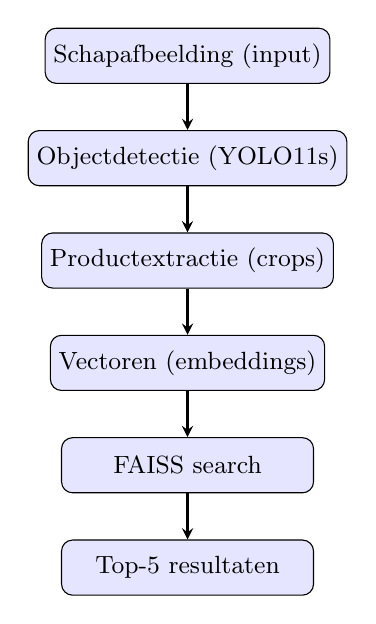
\begin{tikzpicture}[node distance=1.3cm, font=\small]
    \tikzset{
        box/.style={rectangle, rounded corners,
        minimum width=3.2cm, minimum height=0.7cm,
        inner sep=3pt, text centered,
        draw=black, fill=blue!10},
        arrow/.style={thick,->,>=stealth}
    }

    \node (img) [box] {Schapafbeelding (input)};
    \node (yolo) [box, below of=img] {Objectdetectie (YOLO11s)};
    \node (crops) [box, below of=yolo] {Productextractie (crops)};
    \node (emb) [box, below of=crops] {Vectoren (embeddings)};
    \node (faiss) [box, below of=emb] {FAISS search};
    \node (top) [box, below of=faiss] {Top-5 resultaten};

    \draw [arrow] (img) -- (yolo);
    \draw [arrow] (yolo) -- (crops);
    \draw [arrow] (crops) -- (emb);
    \draw [arrow] (emb) -- (faiss);
    \draw [arrow] (faiss) -- (top);
\end{tikzpicture}
}

\end{minipage}
\hfill

\begin{minipage}[t]{0.65\linewidth}
\centering

\includegraphics[width=0.3\linewidth]
{C:/Users/krist/OneDrive/Documents/HoGent IT/BachproefHoGent/latex-hogent-bachproef/bachproef/datasets/SKU-110K_fixed/images/test_0.jpg}
\includegraphics[width=0.11\linewidth]
{C:/Users/krist/Downloads/crop_ex1.jpg}
\includegraphics[width=0.9\textwidth]
{C:/Users/krist/Downloads/crop4_top5.jpg}

\end{minipage}

\captionof{figure}{fgjfdnhgjkflsghnkshgndfgjkdfnsfdkjgnfgfkgjnj}
\end{minipage}


Gedetecteerde producten werden uitgesneden tot crops, waarna multimodale embeddings werden gegenereerd met CLIP, OCR via Florence-2 en Florence-2 visual. Productmatches werden gezocht via FAISS similarity search op een OpenFoodFacts-referentiedataset. 

De experimenten onderzochten de impact van fine-tuning van YOLO11s op SKU-110K, de impact van fine-tuning van CLIP op OpenFoodFacts, verschillende combinaties van CLIP-, OCR- en Florence-2-embeddings, de invloed van verschillende embeddinggewichten enachtergrondverwijdering als mogelijke verbetering van productmatching. 

% \section{Sectie met figuur}

% De {\LaTeX} figure-omgeving bepaalt zelf waar een afbeelding komt en dat is meestal niet op de plek in de tekst waar de figure-omgeving gedefinieerd wordt. Als je wilt forceren dat afbeeldingen toch in de flow van de tekst blijven, dan kan je dat zoals hieronder:

% \begin{center}
%   \captionsetup{type=figure}
%   \includegraphics[width=1.0\linewidth]{grail}
%   \captionof{figure}{He hasn't got shit all over him. The nose? Where'd you get the coconuts? What do you mean? We shall say `Ni' again to you, if you do not appease us}
% \end{center}

% Let er wel op dat dit tot problemen met bladschikking kan leiden.

\section{Conclusies} 

Fine-tuning bleek essentieel voor productdetectie in supermarktbeelden. Het gefinetunede YOLO11s-model behaalde aanzienlijk betere detectieresultaten dan het basismodel en vormde geen belangrijke bottleneck meer binnen de pipeline. Voor productidentificatie leverde de combinatie van CLIP- en OCR-embeddings de beste resultaten op. 

Tekstinformatie afkomstig van verpakkingen bleek cruciaal voor het onderscheiden van sterk gelijkende producten, terwijl Florence-2 visual weinig meerwaarde bood. Hoewel de pipeline vaak relevante producten in de top-5 resultaten terugvond, bleef betrouwbare top-1 identificatie op SKU-niveau moeilijk. 

De grootste uitdaging ligt daardoor niet langer bij objectdetectie, maar bij similarity-based matching tussen visueel sterk gelijkende producten. De resultaten tonen aan dat automatische assortimentsinventarisatie technisch haalbaar is, maar dat verdere verbeteringen nodig zijn voor betrouwbare SKU-level productherkenning in realistische retailomgevingen.

\section{Toekomstig onderzoek}

Toekomstig onderzoek kan zich richten op het gebruik van meer gespecialiseerde vision-language modellen voor productherkenning in retailomgevingen. 

Daarnaast kunnen verbeteringen in productsegmentatie en cropkwaliteit bijdragen aan nauwkeurigere embeddings en productmatches. 

Ook de uitbreiding en kwaliteitsverbetering van referentiedatasets biedt mogelijkheden om de prestaties verder te verhogen. 

Ten slotte is verdere validatie op beelden uit Vlaamse supermarkten nodig om de praktische inzetbaarheid van de voorgestelde pipeline voor automatische assortimentsinventarisatie te onderzoeken.

\end{multicols}
\end{document}